%--------------------
% Packages
\documentclass[12pt,a4paper]{report}
\usepackage[utf8]{inputenc}

\usepackage[sorting = none]{biblatex}
\addbibresource{references.bib} %Import the bibliography file

\usepackage{fancyhdr}
\usepackage[pdftex]{graphicx} % Required for including pictures
\usepackage[pdftex,linkcolor=black,pdfborder={0 0 0}]{hyperref}
\usepackage{parskip}
\usepackage{comment} % delete when publishing
\usepackage[nottoc]{tocbibind}
\usepackage{tocloft}
\usepackage{tabularx}
\usepackage{listings}
\usepackage{array}
\usepackage[rightcaption]{sidecap}
\pagestyle{fancy}\fancyhf{}
\fancyhead[LE]{\nouppercase{\rightmark\hfill\leftmark}}
\fancyhead[RO]{\nouppercase{\leftmark\hfill\rightmark}}
\fancyfoot[LE,RO]{\hfill\thepage\hfill}
\def\aruco{ArUco }
% -------------------
\author{Sharan Govinden Umavassee}
\title{Low-cost vision system for autonomous outdoor robots}
\date{December 2022}

\begin{document}
\pagenumbering{roman}
\begin{titlepage}
\centering
{\Large\textsc University of Southampton\par}
{\Large\textsc School of Electronics and Computer Science\par}
{\Large\textsc Faculty of Physical Sciences and Engineering\par}
\vspace{3cm}
{\huge\bfseries Low-cost vision system for autonomous outdoor robots\par}
\vspace{2.5cm}
{\Large\itshape \textsc{Umavassee} Sharan Govinden\par}
{\Large 31248551 $|$ sgu1n19@soton.ac.uk\par}
\vspace{2cm}
{\Large Project Supervisor: \itshape Dr. Klaus-Peter Zauner\par}
{\Large Second Examiner: \itshape Prof. Christopher Freeman\par}
\vfill
% Bottom of the page
{\large {A project progress report submitted for the award of
\\MEng Computer Science with Industrial Studies}\par}
\vspace{1cm}
{\large May 2023}
\end{titlepage}

\tableofcontents

\clearpage
\listoftables
\listoffigures
\clearpage

\chapter{Introduction}
\pagenumbering{arabic}
The field of computer vision has experienced tremendous growth over the past few decades, driven by advancements in machine learning, digital image processing, and camera technology \cite{szeliski2010computer}\cite{lecun2015deep}. One of the key applications of computer vision is in navigation systems, where the ability to detect and recognise objects in real-time is critical for guiding autonomous vehicles, robots, or even humans in complex environments \cite{thrun2005probabilistic}\cite{bonin2008visual}.

Fiducial markers, often utilized in augmented reality applications, are artificial landmarks that can be easily detected and tracked by computer vision algorithms \cite{kato1999marker}. These markers provide robust and reliable reference points, encoded in a planar pattern enabling reliable detection in images, accurate pose estimation and facilitating navigation in both indoor and outdoor environments \cite{garrido2014automatic}. \aruco markers, a specific type of fiducial markers, are square-shaped patterns with a unique identification code that allows for rapid detection and decoding \cite{garrido2016generation}.

In this project, we present the development and implementation of an \aruco gate detection system for computer vision-based navigation. The primary objective of this project is to create a system capable of accurately detecting and recognizing ArUco markers arranged in a gate-like configuration, estimating their relative position and alignment, and providing navigation information to guide autonomous robots through these gates. This project has the potential to impact various fields, including robotics, unmanned aerial vehicles (UAVs), and indoor navigation systems \cite{boniardi2016autonomous}.

To achieve this objective, we leverage the power of the OpenCV library, a widely-used open-source computer vision library that provides a rich set of tools and algorithms for image processing and computer vision tasks \cite{bradski2008learning}. OpenCV includes a dedicated module for ArUco marker detection and decoding, which forms the basis of our ArUco gate detection system \cite{romero2018speeded}.

In the following sections, we will provide a detailed literature review on fiducial markers, ArUco markers, and computer vision-based navigation. We will then present our methodology, outlining the algorithms and techniques employed in the development of the system. Finally, we will discuss the implementation, results, limitations, and future work to further enhance the system's capabilities and applications.

By the end of this dissertation, we aim to provide a comprehensive understanding of fiducial marker systems and \aruco gate detection systems and their potential use in computer vision-based navigation, opening new avenues for research and development in this rapidly evolving field.

\chapter{Background}
\label{Chapter: Background}
\section{Fiducial Markers}
\label{sec: Fiducial Markers}
%What are Fiducial markers?
Fiducial markers refer to artificial landmarks added to a scene to facilitate locating point correspondences between images, or between images and a known model \cite{reliablefiducialmarkers}. They are 2D binary black and white patterns that computer vision algorithms can easily detect.

%How are they useful?
They are useful when object recognition or pose determination is needed with high reliability and when natural features are insufficient in quantity and uniqueness. Fiducial markers also offer a highly distinguishable pattern and have an encoding that acts as a fail-safe against misdetections. They provide a robust and reliable means of determining the camera pose in relation to the marker, enabling accurate position and orientation estimation in real-time.
Their applications include augmented reality (AR), input devices for human-computer interaction (HCI) and robot navigation \cite{reliablefiducialmarkers}. They are attractive because of their high reliability and small size.

% Types of markers
Various types of fiducial markers exist, including square markers, circular markers, and natural feature markers. Among these, square markers have been widely used due to their simple geometric structure and ease of detection. The most commonly used fiducial markers are ARTag \cite{artag}, AprilTag \cite{apriltag}, ARToolKit \cite{artoolkit}, \aruco \cite{garrido2014automatic} and STag \cite{stag}, as shown in \autoref{fig:Figure 1} from \textbf{a} to \textbf{d}.\\
Most square shaped marker frameworks are based on ARToolKit \cite{artoolkit}, initially created for AR video conferences \cite{kato1999marker}. ARtag is based on ARToolKit but uses digital coding theory to create the marker’s internal pattern \cite{FMforposeestimation}.

\begin{figure}[h]
    \centering
    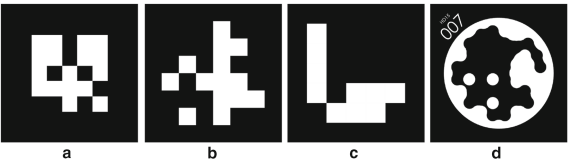
\includegraphics[width=1\textwidth]{Images/markers.png}
    \small \caption[Types of Fiducial Markers]{Types of Fiducial Markers: \textbf{a} ARTag, \textbf{b} AprilTag, \textbf{c} \aruco, \textbf{d} STag. Reproduced from \cite{FMforposeestimation}}
    \label{fig:Figure 1}
\end{figure}

AprilTag and \aruco are both instances of marker systems that build on the ARTag framework. They each offer several improvements on the framework.\\
AprilTag introduced a graph-based image segmentation algorithm that analyses gradient patterns on images and a new programming system to take care of issues stemming from the 2D barcode system. Because they deal with the issues of incompatibility with rotation and false positives in outdoor applications, AprilTags provide high robustness against occlusion and warping and a decreased quantity of misdetections \cite{FMforposeestimation}.

\aruco markers, similar to their "sibling frameworks", offer the possibility of using predefined libraries. However, their major feature is that they allow users to create configurable libraries. This allows users to generate custom libraries based on their specific needs and only comprising markers with maximum Hamming distance \cite{FMforposeestimation}---the distance between two binary vectors of equal length, that is, the number of positions at which the corresponding bits in the patterns are different \cite{ALTAWELL202247}. ArUco's capacity to create custom libraries of desired length removes the need to include all possible markers in standard libraries, hence offering a low-computational cost.

A number of studies \cite{comparearandapriltag}\cite{compareartagartoolkitplus} have compared the different fiducial marker systems available. In Michail Kalaitzakis et al.'s paper \cite{FMforposeestimation}, the authors experimented on the following monochromatic and square shaped frameworks: ARTag, AprilTag, \aruco and STag \cite{stag}. They tested performance metrics such as varying marker distance, varying marker orientation, motion blur and computational cost. \autoref{tab:Table 1} displays a summary of the results obtained from the experiments carried out outlining the advantages and disadvantages of each marker system.

\begin{table}[h]
    \centering
    \caption[Advantages and disadvantages of fiducial marker packages]{Main advantages and disadvantages of the four evaluated packages in Michail Kalaitzakis et al.'s paper \cite{FMforposeestimation}}
    \label{tab:Table 1}
    {\footnotesize
    \begin{tabularx}{\textwidth}{|p{0.12\textwidth}|p{0.392\textwidth}|p{0.392\textwidth}|}
        \hline
        Marker & Advantages & Disadvantages \\
        \hline
        ARTag & - Lowest computational cost & - Low detection rate for single markers \\
        & & - Extreme outliers \& high standard deviation in marker bundles \\
        \hline
        AprilTag & - Great orientation results  & - Most computationally expensive \\
        & - Great detection rate & - Most sensitive to motion blur\\
        & - Good position results & - Worst results in the non-planar setup\\
        \hline
        \aruco & - Good position results  & - Sensitive to smaller marker sizes \\
        & - Great detection rate & - Sensitive to larger distances \\
        & - Low computational cost for single markers & - Computational cost scales with multiple markers\\
        & - Good orientation results & \\
        \hline
        STag & - Great position results and detection rate & - Sensitive to smaller marker sizes and larger distances \\
        & - Good orientation results & \\
        \hline
    \end{tabularx}
    }
\end{table}

\section{\aruco Markers}
\label{section 2.2: aruco markers}
\aruco markers have gained popularity in computer vision applications due to their simplicity, robustness, ease of detection and rapid decoding. These black and white square binary patterns provide a balance between efficiency and accuracy, allowing for rapid and reliable marker identification and tracking. ArUco markers are invariant to scale, rotation, and illumination changes, which makes them suitable for real-time applications like augmented reality, robotics, and navigation \cite{garrido2014automatic}. They can be easily generated, and their size and pattern can be customized to suit specific requirements. Additionally, \aruco markers support error detection and correction, further enhancing their reliability in challenging conditions in outdoors environment such as lighting variations and camera motion blur.

\aruco markers have been used in a wide range of applications, such as robot localisation and tracking \cite{garrido2014automatic}. In robotics, ArUco markers have been employed to localise robots within their environment, facilitating navigation tasks and improving overall system performance \cite{gil2010}. In unmanned aerial vehicles (UAVs), ArUco markers have been utilized for precision landing and way-point navigation \cite{marut2019}. The use of ArUco markers in augmented reality applications enables the overlay of virtual objects onto real-world scenes, enhancing user experience and interaction \cite{kato1999marker}\cite{wagner2008}.

\newpage
\section{Marker Detection}
\label{2.3 Marker Detection}
This section explains how to detect the markers in an image using OpenCV \cite{bradski2008learning}. We aim at extracting the binary code from the detected square markers.

OpenCV  is a widely-used open-source computer vision library that provides a comprehensive set of tools and algorithms for image processing and computer vision tasks \cite{opencvabout}\cite{bradski2008learning}. Example applications: to detect faces or identify objects in an image and classify human actions in videos.

OpenCV includes a dedicated module for ArUco marker detection \cite{opencvdetectionaruco} and decoding \cite{opencvarucomodule}\cite{opencvaruco}, making it an ideal choice for this project. The ArUco detection module in OpenCV employs the fast corner detection algorithm and adaptive thresholding for robust marker detection \cite{garrido2016generation}.

\begin{SCfigure}[1][ht]
    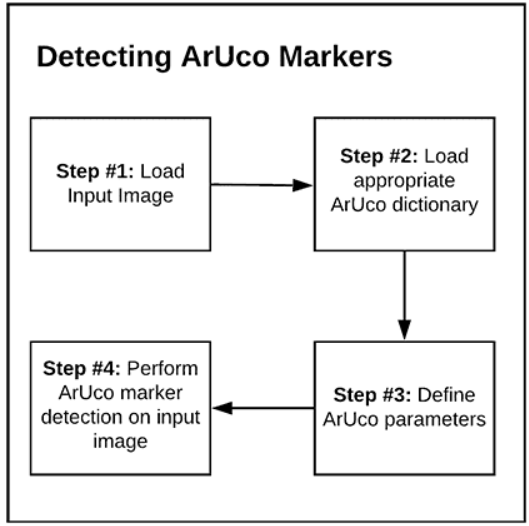
\includegraphics[width = 0.55\textwidth]{Images/detectaruco.png}
    \caption[Flowchart of steps required to detect \aruco markers]{Flowchart of steps required to detect \aruco markers with OpenCV.\\Reproduced from \cite{pyimagesearch}}
    \label{fig: Figure 2}
\end{SCfigure}

Marker dictionaries, or libraries, broadly refer to a set of a specific type of markers. We use them to generate and detect \aruco markers. There are 21 different ArUco dictionaries built into the OpenCV \aruco dedicated module. They are categorised based on number of bits and number of markers in the dictionary, ranging from 50 to 1000. The NxN value is the 2D bit size of the \aruco marker. The integer M following the grid size specifies the total number of unique \aruco IDs that can be generated with the dictionary.

\aruco markers can be generated through code or generator tools such as the ArUco Marker Generator project by Oleg Kalachev obtained through their open-source github project \cite{arucogenerator}.

\newpage
A predefined \aruco dictionary with 50 markers with bit size 4X4:
\begin{lstlisting}[language=Python, frame=single]
cv2.aruco.Dictionary_get(cv2.aruco.DICT_4X4_50)
\end{lstlisting}

As mentioned in \autoref{sec: Fiducial Markers}, the \aruco marker system also offers the possibility to create configurable libraries to adhere to the user's specific needs. The method cv2.aruco.Dictionary\_create(X, Y) takes two parameters X and Y and creates a customised dictionary composed of X markers of YxY bits. In cases where we require less than 50---the minimum number of markers available in predefined dictionaries---or a specific number of unique markers, the \aruco marker system greatly helps as it heavily reduces the computational cost \cite{FMforposeestimation}.

Markers from the customised dictionary have maximum Hamming distance between them. The Hamming distance between two equal-length strings of symbols is defined as the minimum number of errors or substitutions that can transform one string into the other \cite{hammingdistancedefn}. In simpler terms, it is the difference in bits between two bit sequences. This ensures that the markers will be distinguishable from one another considering variables in the environment or algorithm that might impact the detection of markers.

\textbf{Detection process of \aruco markers for custom dictionaries\\}
Generate custom dictionary of 4 \aruco markers with bit size 4X4:
\begin{lstlisting}[language=Python, frame=single]
arucoDict = cv2.aruco.Dictionary_create(4,4)
arucoParams = cv2.aruco.DetectorParameters_create()
\end{lstlisting}
Detect ArUco markers in the image frame:
\begin{lstlisting}[language=Python,frame=single]
(corners, ids, rejected) = cv2.aruco.detectMarkers(
frame,arucoDict, parameters=arucoParams)
\end{lstlisting}

After performing the \aruco marker detection algorithm, we obtain three key information that helps us identify the marker:\\
\textbf{\textit{corners:}} a list containing the (x,y)-coordinates of the detected \aruco markers' corners\\
 \textbf{\textit{ids:}} a list of IDs of the detected markers\\
\textbf{\textit{rejected candidates:}} a list of potential markers that were found but rejected due to the inner code of the marker being unable to be parsed
\newpage
The steps involved in the detection process \cite{garrido2014automatic} are:\\
\textbf{Image Segmentation:} extracts the most important contour using a local adaptive thresholding approach\\
\textbf{Contour extraction and filtering:} obtains the polygons in the marker image\\
\textbf{Marker Code extraction:} extracts the internal code from the inner regions of the extracted contours\\
\textbf{Marker identification and error correction:} determines which marker candidates obtained belongs to the dictionary

\begin{figure}[h]
    \centering
    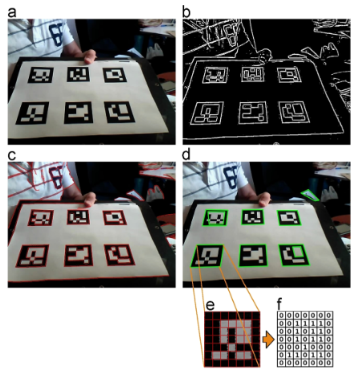
\includegraphics[width=0.85\textwidth]{Images/Image detection process.png}
    \caption[Image process for automatic marker detection]{Image process for automatic marker detection. (a) Original image. (b) Result of applying local thresholding. (c) Contour detection. (d) Polygonal approximation and removal of irrelevant contours. (e) Perspective transformation. (f) Bit assignment for each cell. Reproduced from \cite{garrido2014automatic}}
    \label{fig:Figure 3}
\end{figure}

\section{Computer Vision-based Navigation}
Computer vision-based navigation leverages the power of image processing and computer vision algorithms to guide autonomous agents through complex environments \cite{davison2007}. The use of fiducial markers, such as ArUco markers, has been shown to improve navigation performance by providing accurate reference points.

Despite the advantages of computer vision-based navigation, several challenges remain to be addressed. These challenges include occlusion, lighting variations, and camera motion blur, which can affect the detection and decoding of fiducial markers \cite{sattler2011}\cite{maggio_cavallaro_2011}. To overcome these challenges, various approaches have been proposed, such as adaptive thresholding, multi-scale detection, and robust estimation techniques \cite{garrido2016generation}.

The research literature demonstrates the potential of ArUco markers in facilitating computer vision-based navigation tasks. By understanding the existing research and techniques, we can develop and implement an effective ArUco gate detection system as part of this project. The following sections of this dissertation will detail the methodology, system design, implementation, and evaluation of the proposed project.

\chapter{Methodology}
\label{Chapter: Methodology}
This section proposes and describes the methodology and concepts behind the project. We aim to create a low cost computer vision-based navigation system for outdoor autonomous robots.
We set fiducial markers, acting as gates, on a path and the vision system will provide the robot with navigational/directional information.

The \aruco marker system is selected as our fiducial markers because of its low computational cost, great detection rate in real-time applications and configurable dictionary functionality and reliability in challenging outdoor conditions as mentioned in \autoref{section 2.2: aruco markers}. The black and white pattern, enabling rapid detection and decoding, allows for a greater chance for real-time detection on a small low-cost computer.

A customised dictionary, made for the project's specific purpose, of 4 \aruco markers with 4x4 bit size is generated, as shown in \autoref{2.3 Marker Detection}. Using the four-by-four bit size, the smallest marker bit size available for ArUco, offers a bigger and more distinguishable pattern. The four markers required are the two directional markers: left and right markers, and the start and stop markers.
\autoref{fig:Figure 4} shows the four \aruco markers generated by our custom dictionary. Each \aruco ID is appointed to a specific marker for uniqueness. The configurable dictionary and small number of tags provide markers with the maximum Hamming distance, helping to make them distinguishable from one another, which reduces chances of misdetection and false positives \cite{FMforposeestimation}.

OpenCV allows us to use computer vision algorithms to load and process the image frames and, with its \aruco detection module, enables us to generate the custom dictionary and detect the markers as explained in \autoref{2.3 Marker Detection}.

\begin{figure}[h]
    \centering
    
\includegraphics[width=1\textwidth]{Images/ArUco tags hori.png}
    \caption[Selected \aruco tags]{Selected \aruco tags generated by custom dictionary: \textbf{a} left, \textbf{b} right, \textbf{c} start, \textbf{d} stop markers.}
    \label{fig:Figure 4}
\end{figure}

The process is described as follows:\\
Once the start tag is detected, the vision system will start looking for the two directional markers. A gate is formed if two detected markers are left and right markers, in parallel, have approximately the same edge size and are in their correct respective positions---left marker on the left and right marker on the right, as shown in \autoref{fig:Figure 5}. \autoref{fig:Figure 6} displays card designs for each \aruco tag, made from previous work \cite{elias}.

\begin{figure}[h]
    \centering
    
\includegraphics[width=0.75\textwidth]{Images/Gate Formation.png}
    \caption[Formation of Gates]{Formation of Gates: using the Left and Right \aruco markers}
    \label{fig:Figure 5}
\end{figure}

\begin{figure}
    \centering
    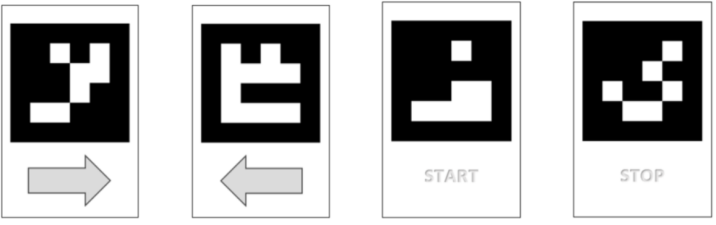
\includegraphics[width=1\textwidth]{Images/Tags on card.png}
    \caption[Marker Card Design]{Marker Design: The cards include the markers from \autoref{fig:Figure 5} and a visual aid that helps setting up the path correctly.}
    \label{fig:Figure 6}
\end{figure}

A list of detected markers is created and sorted by size of marker to obtain the closest tags relative to the camera. The closest markers are checked against the gate requirements. The system then computes the target point by calculating the middle point of the diagonal length across the furthest corners of the two markers. This target point is then used as reference with the camera centre point to calculate the direction to guide the robot towards.

\newpage
A Raspberry Pi can be used to run the navigation system which will provide the robot with directional instructions. This can be done in two ways:
\begin{enumerate}
    \item through its General-Purpose Input/Output (GPIO) pins---one pin to go straight, one pin to go left and one pin to go right.
    \item over UART serial connection---encoding the target point's x-coordinate as an ASCII value scaled using a factor of 25 divided by the width of the image frame, representing all alphabets from A to Z.
\end{enumerate}

The methodology demonstrates the concepts that would be used in implementing the computer vision-based navigation system. By understanding the marker design and setup techniques, we can effectively carry out steps in our implementation phase in the following section.

\begin{comment}
    Explain process:
- Detect left and right marker \\
- identifies closest markers through sorting list of markers by size \\
- what 2 markers form a gate?: left marker on left, right marker on right, appear to be parallel \\
- looks at marker edge size and see if left and right marker have approximately the same size \\
- may be difference because of distortion in image and convection in lens: angle is different hence may be perceived length is different

Once gate has been identified, \\
- system computes the centre of gate and aims for that\\
- calculate how to change direction from current image stream to desired image stream -> that is move towards target point\\
- outputs directional information\\
- method of output -> pings on raspberry pi to go left, right, straight
\end{comment}

\chapter{Implementation}
\label{Chapter: Implementation}
The project implementation is done in two parts: for high and low processing machines. The high processing implementation is done on a computer having an 8-core CPU and using the Windows operating system. The low processing implementation---the desired outcome of this project---is done on a single core Raspberry Pi Zero \cite{raspberrypizero}. The processes were adapted to the specific machines.

\section{Windows Implementation}

\section{Raspberry Pi Implementation}
This project uses a Raspberry Pi Zero, a camera, the OpenCV library and a detection algorithm for fiducial markers. The detection algorithm process, written in Python, is described below.

Up to this point, the progress made in this project was the study of theoretical and technical concepts: fiducial markers, computer vision, OpenCV and Python, and the implementation of a prototype on larger resource computer.

The first stage of the project was focused on research. Academic papers about fiducial markers \cite{garrido2014automatic}\cite{FMforposeestimation} were read and I studied computer vision in the COMP3204 module of University curriculum of 2022-2023. Technical software topics like OpenCV and Python were also studied using programming tutorials \cite{pyimagesearch} and document reading \cite{opencvarucomodule}.

The following stage involved the implementation of a prototype of the system that would work on a larger resource machine---a personal computer with the Windows 10 Operating System. Since the \aruco library in OpenCV is freely available on Python, there was no need to implement the system on another operating system, thus removing possible compatibility issues.

The prototype system uses a top-down approach where large tasks are broken into a series of smaller ones. The small tasks are then created first and merge together to form the bigger blocks.
First, we use the OpenCV library to load and process an image. The detection of \aruco markers was done in two part---using predefined dictionaries to detect markers in an image and a video stream and generating a customised dictionary suiting our specific needs.

The predefined \aruco dictionary used was cv2.aruco.DICT\_4X4\_50, providing 50 markers of four-by-four bit size. After doing the detection process as mentioned in \autoref{Chapter: Methodology}, the detected markers' ID, borders and centre point are highlighted with the marker ID written in green at the top left, green edges and a red circle respectively as shown in \autoref{fig:Figure 7}.

\begin{figure}[ht]
    \centering
    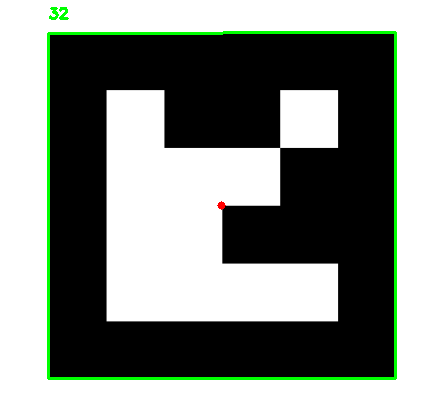
\includegraphics[width=0.5\textwidth]{Images/ArUco marker id 32 detection test.png}
    \caption[Detection test on \aruco marker]{Detection test on \aruco marker with ID 32 from dictionary cv2.aruco.DICT\_4X4\_50 }
    \label{fig:Figure 7}
\end{figure}

The next part of the prototype system implementation is to allow the algorithm to detect markers using a camera feed. This can easily be done using OpenCV library to connect to the camera and load and loop over the video stream and detect the markers over the looped frames.  This part also involved generating the custom dictionary to detect the 4 marker cards. An example of the detected marker through a camera feed is shown in \autoref{fig:Figure 8}.

\begin{figure}[ht]
    \centering
    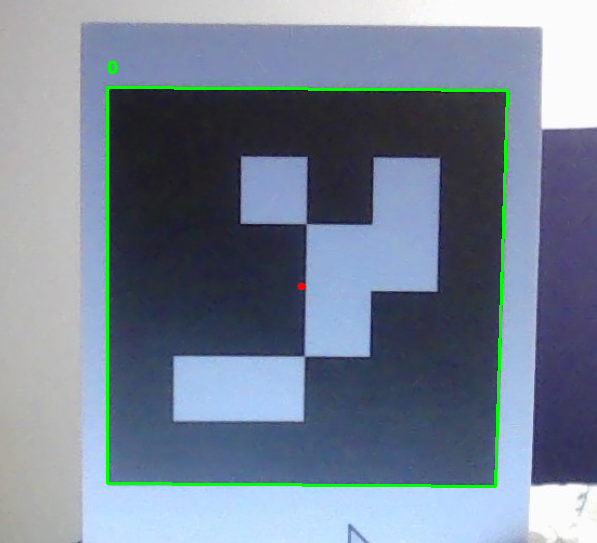
\includegraphics[width=0.5\textwidth]{Images/left marker detection test.png}
    \caption[Detected marker of custom \aruco dictionary]{Detected marker of custom \aruco dictionary with marker ID 0, left marker, through camera feed}
    \label{fig:Figure 8}
\end{figure}

The next stage of the project is to continue the implementation of the prototype system by computing the target point to navigate towards and calculating the directional changes and directional outputs to be given to the robots. Following this, we will translate this detection and navigation algorithm onto a Raspberry Pi Zero. Further research needs to be done on microcontrollers and embedded systems.

\chapter{Project Management}
\label{Chapter: Project Management}
Project management was carried out with the help of a project management tool---Asana \cite{asana}---and a note taking and organisational workspace application--- Notion \cite{notion}. Asana was used to list and organise tasks, give priority to tasks and provide overview of project. Notion was used to organise a working schedule for the project, brainstorm ideas, write notes from research done and plan for the report.

To manage the project, a break down of tasks was carried out and uploaded on Asana. Each task was given a priority level between Low, Medium and High to allow for sufficient timing for research and implementation and tailor to the progress report deadline on Tuesday 13$^{th}$ December 2022 and final report deadline Tuesday 3$^{rd}$ May 2023. The tasks were organised in a list of To-do, Done and Doing and were interchanged between the different lists based on the current stage of implementation. Some tasks were given deadlines to better accommodate to the timelines. \autoref{fig:Figure 9} displays the project management board on Asana containing list of tasks organised into to-do lists their priority levels.

My project supervisor Dr. Klaus-Peter Zauner, whom I would like to thank, and I have set up weekly recurring hour-long meetings every Tuesday at 15:00 to discuss on the project progress. This allowed me to gain direct insights into the project using his invaluable expertise on the subject of robotics and computer vision. He was an incredible help with structuring the project progress and guiding me throughout the prototype implementation and theoretical concepts.

\begin{figure}[t]
    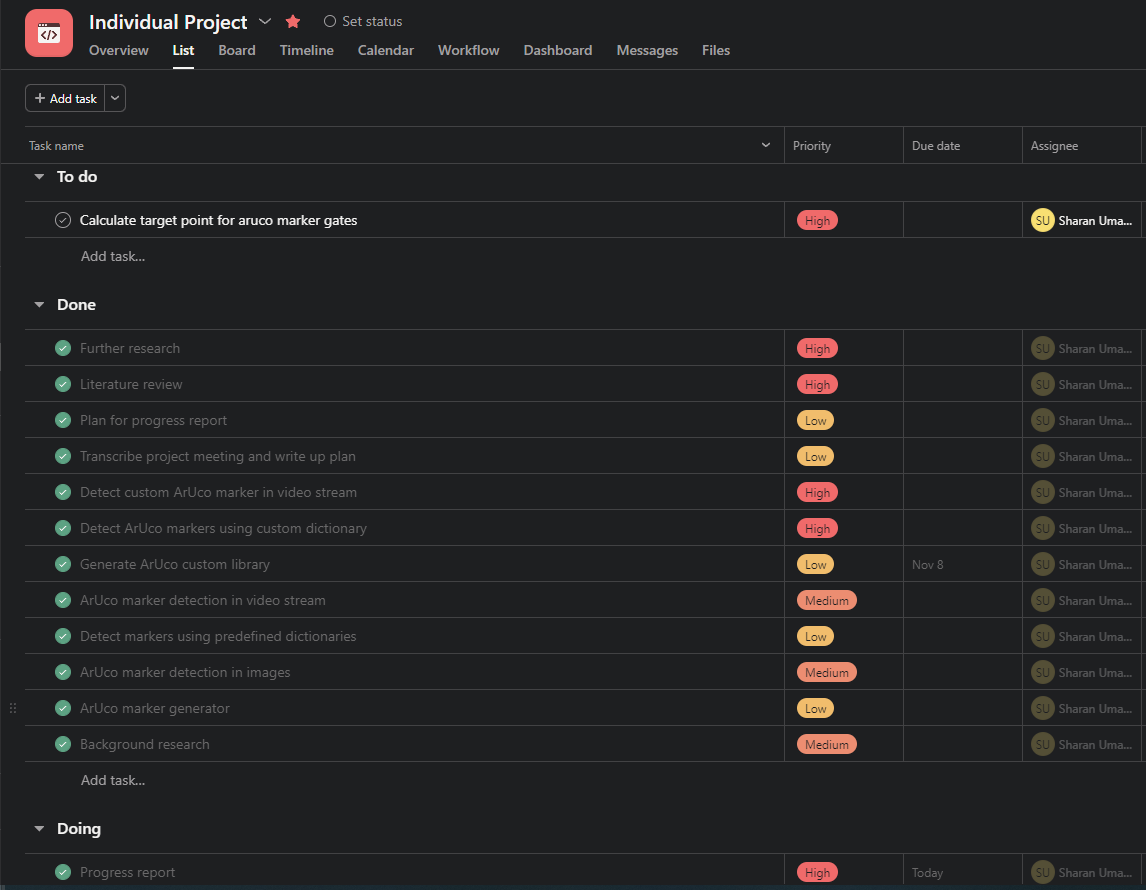
\includegraphics[width = 1\textwidth]{Images/Asana.png}
    \caption[Asana Project management board]{Asana Project management board displaying list of tasks organised into to-do lists and given a priority level (Low, Medium, High)}
    \label{fig:Figure 9}
\end{figure}

\newpage
\printbibliography[heading=bibintoc,title={References}] %Prints bibliography

\end{document}